\section{Introdução}

O objetivo deste trabalho é detalhar várias etapas da análise de sistemas em tempo discreto, bem como realizar o projeto de controladores e observadores de estado. Para isso são utilizadas duas plantas, uma BIBO estável e outra BIBO instável, para haver uma comparação e abordagem de uma quantidade maior de paradigmas ao lidar com essas plantas.

\subsection{Sistemas a serem trabalhados}

As plantas a serem trabalhadas são baseadas em exemplos básicos de funções de transferência da literatura de controle e estão representadas no domínio da frequência pela transformada de Laplace. A primeira é uma planta (\ref{g:est}) estável de segunda ordem e bastante oscilatória. Enquanto que a segunda é uma planta (\ref{g:ins}) de segunda ordem instável com dois polos diferentes, incluindo um na origem. 

\begin{equation} \label{g:est}
    G_{est}(s) = \frac{10}{(s^2+2s+25)}
\end{equation}

\begin{equation} \label{g:ins}
    G_{ins}(s) = \frac{2}{s(s+0.5)}
\end{equation}


\subsection{Discretização por ROZ}

Para realizar a discretização por retentor de ordem zero (ROZ) das plantas é necessário transformar a representação em função de transferência no domínio da frequência em uma representação por equação diferencial e logo após para uma representação no tempo em espaço de estados. Após obter a representação por espaço de estados em tempo contínuo, realiza-se a discretização e obtém-se a representação por espaço de estados em tempo discreto. 

\subsubsection{Representação em espaço de estados em tempo contínuo}

A forma padrão da representação em espaço de estados em tempo contínuo segue as equações \ref{est_sp}:

\begin{equation} \label{est_sp}
\centering
\left \{
\begin{array}{cc}
\Dot{\textbf{x}}(t) = \textbf{Ax}(t) + \textbf{B}u(t) \\
y(t) = \textbf{Cx}(t) + \textbf{D}u(t)\\
\end{array}
\right.
\end{equation}

Onde $\textbf{x}(t)$, $\textbf{y}(t)$ e $\textbf{u}(t)$ são, respectivamente, os vetores de estados, saídas e entradas. As matrizes $A$, $B$, $C$ e $D$ são, respectivamente, a matriz de transição de estados, de entradas, de saídas e de transmissão direta. (LATHI, 2005)

Considerando a planta estável, ao expandir sua FT obtém-se:

\begin{equation} \label{est:1}
    (s^2+2s+25)Y(s) = 10U(s)
\end{equation}

Considerando condições iniciais nulas, ao aplicar a transformada inversa de Laplace na equação \ref{est:1}, obtém-se a seguinte 

\begin{equation} \label{est:2}
    \ddot{y}(t) + 2\dot{y}(t) + 25y(t) = 10u(t)
\end{equation}

Considera-se o sistema de equações \ref{est:3} para os estados:

\begin{equation} \label{est:3}
\centering
\left \{
\begin{array}{cc}
x_1 = y \\
x_2 = \dot{y}\\
\end{array}
\right.
\end{equation}

Obtém-se:

\begin{equation} \label{est:4}
\centering
\left \{
\begin{array}{cc}
\dot{x_1} = x_2 \\
\dot{x_2} = \ddot{y} = 10u - 25x_1 - 2x_2\\
\end{array}
\right.
\end{equation}

Assim as matrizes da representação em espaço de estados serão:

\begin{equation} \label{est:5}
    A = \begin{bmatrix} 0 & 1 \\ -25 & -2  \end{bmatrix}; B = \begin{bmatrix} 0 \\ 10 \end{bmatrix}; C = \begin{bmatrix} 1 & 0  \end{bmatrix}; D = 0
\end{equation}

O processo é análogo para a planta instável e com as mesas considerações. Sendo a equação \ref{ins:1} a FT expandida, a equação \ref{ins:2} a equação diferencial, o sistema de equações \ref{ins:3} as atribuições dos estados levando em consideração a equação \ref{est:3} e, por fim, as matrizes da representação de estados na equação \ref{ins:4}

\begin{equation} \label{ins:1}
    (s^2+0.5s)Y(s) = 2U(s)
\end{equation}

\begin{equation} \label{ins:2}
    \ddot{y}(t) + 0.5\dot{y}(t) = 2u(t)
\end{equation}

\begin{equation} \label{ins:3}
\centering
\left \{
\begin{array}{cc}
\dot{x_1} = x_2 \\
\dot{x_2} = \ddot{y} = 2u - 0.5x_2\\
\end{array}
\right.
\end{equation}

\begin{equation} \label{ins:4}
    A = \begin{bmatrix} 0 & 1 \\ 0 & -0.5 \end{bmatrix}; B = \begin{bmatrix} 0 \\ 2 \end{bmatrix}; C = \begin{bmatrix} 1 & 0  \end{bmatrix}; D = 0
\end{equation}

\subsubsection{Representação em espaço de estados em tempo discreto}

Encontradas as devidas matrizes dos sistemas, resta discretizar os sistemas para que eles obedeçam a relação da equação \ref{disc:1}.

\begin{equation} \label{disc:1}
\centering
\left \{
\begin{array}{cc}
x[n+1] = \Phi x[n] + \Gamma u[n] \\
y[n] = C x[n] + D u[n]\\
\end{array}
\right.
\end{equation}

Onde a matriz de transição de estados é $\Phi = e^{Ah}$, a matriz de entradas é $\Gamma = \int_{0}^{h} e^{At} B dt$ e $h$ é o período de amostragem. Durante a análise, a forma de resolver $e^{Ah}$ irá obedecer a equação \ref{disc:2} (transformada inversa de Laplace da matriz inversa de $sI-A$) e os cálculos de $\Phi$ e $\Gamma$ ficarão em função de $h$ e serão agilizados por meio de \textit{softwares} computacionais, como Scilab e Wolfram Alpha.

\begin{equation} \label{disc:2}
    \Phi = \mathcal{L} ^{-1} (sI-A)^{-1}
\end{equation}

Dessa forma, para o sistema estável tem-se que as matrizes $\Phi$ e $\Gamma$ são:

\begin{equation} \label{est:6}
    \Phi= \begin{bmatrix} e^{-h} \left(\frac{sen(2\sqrt{6}h)+2\sqrt{6}cos(2\sqrt{6}h)}{2\sqrt{6}}\right) & e^{-h}\frac{sen(2\sqrt{6}h)}{2\sqrt{6}}\\ -25e^{-h}\frac{sen(2\sqrt{6}h)}{2\sqrt{6}} & e^{-h}\left(\frac{2\sqrt{6}cos(2\sqrt{6}h)-sen(2\sqrt{6}h)}{2\sqrt{6}}\right)\end{bmatrix}
\end{equation}

\begin{equation} \label{est:7}
    \Gamma = \begin{bmatrix} \frac{1}{30} e^{-h}(12e^{h}-\sqrt{6}sen(2\sqrt{6}h)-12cos(2\sqrt{6}h)) \\ 5e^{-h}\frac{sen(2\sqrt{6}h)}{2\sqrt{6}} \end{bmatrix}
\end{equation}

E para o sistema instável tem-se que as matrizes $\Phi$ e $\Gamma$ são:

\begin{comment}
\begin{equation} \label{ins:5}
    \Phi= \begin{bmatrix} 1 & 1.92308(1-e^{-0.52h})\\ 0 & e^{-0.52h} \end{bmatrix}
\end{equation}

\begin{equation} \label{ins:6}
    \Gamma = \begin{bmatrix} 3.84616h + 7.39646e^{-0.52h} - 7.39646\\ 3.84615
    (1-e^{-0.52h}) \end{bmatrix}
\end{equation}
\end{comment}

\begin{equation} \label{ins:5}
    \Phi= \begin{bmatrix} 1 & 2(1-e^{-0.5h})\\ 0 & e^{-0.5h} \end{bmatrix}
\end{equation}

\begin{equation} \label{ins:6}
    \Gamma = \begin{bmatrix} 4(h + 2e^{-0.5h} - 2)\\ 4(1-e^{-0.5h}) \end{bmatrix}
\end{equation}

Finalmente os sistemas estão discretizados.

\subsubsection{Período de amostragem}

A escolha do período de amostragem é essencial para que o sistema discreto represente da melhor maneira possível o sistema contínuo real. Dessarte, este trabalho utilizou a análise a partir da largura de banda limitada pela frequência de corte das funções de transferência (frequência para a qual o módulo da função de transferência é -3dB), de modo que as componentes frequenciais acima desta frequência são deveras atenuadas, permitindo estabelecer esta frequência como a maior permitida no sistema. Para obedecer o teorema de Nyquist e regras de ordem prática, foi adotada uma frequência de amostragem no mínimo quinze vezes maior do que a frequência de corte.

Para encontrar a frequência de corte basta igualar o módulo da função de transferência a -3dB ou 0.5 com $s = j\omega$ e resolver as equações para \ref{wb:1} e \ref{wb:2} $w$. Para facilitar os cálculos, foram determinados os polos das funções de transferência.

\begin{equation} \label{wb:1}
    |G_{est}(j\omega)| = \left |\frac{10}{(j\omega +1-j2\sqrt{6})(j\omega +1+j2\sqrt{6})} \right| = 0.5 
\end{equation}
\begin{equation} \label{wb:2}
    |G_{ins}(j\omega)| = \left |\frac{2}{j\omega(j\omega+0.5)} \right| = 0.5 
\end{equation}

Resolvendo as equações, encontra-se uma frequência de corte para a planta estável de $\omega_{B_{est}} = 6.3588 rad/s$ e de $\omega_{B_{ins}} =  1.969 rad/s$ para a planta instável. 

O período de amostragem será dado pela equação \ref{wb:3} para a planta estável e pela equação \ref{wb:4} para a planta instável, considerando as relações de que $\omega_B = 2\pi f_B$, $f_S = 15f_B$ (para garantir que não haverá \textit{aliasing}) e $h = f_S^{-1}$

\begin{equation} \label{wb:3}
    h_{est} = 0.06587 s \approx 0.01 s 
\end{equation}
\begin{equation} \label{wb:4}
    h_{ins} = 0.2127 s \approx 0.1 s 
\end{equation}

\subsection{Análise das saídas}

Serão avaliadas as saídas dos sistemas para entradas do tipo degrau e senoide em tempo contínuo e discreto à título de comparação.

Considerando a solução no domínio do tempo de equações de estado em tempo contínuo proposta por LATHI (2005) na equação \ref{sol:cont:1}, tem-se que a saída é dada como a componente $x_1$ das variáveis de estado de acordo com o que foi proposto em \ref{est:3}.

\begin{equation} \label{sol:cont:1}
    \textbf{x}(t)= e^{\textbf{A}(t-t_0)}\textbf{x}(t_0) + \int_{t_0}^{t} e^{A(t-\tau)}\textbf{B}u(\tau) d\tau
\end{equation}

Considerando $t_0=0$ e condições iniciais nulas, tem-se que a componente da resposta só depende da resposta forçada:

\begin{equation} \label{sol:cont:2}
    \textbf{x}(t)= \int_{0}^{t} e^{A(t-\tau)}\textbf{B}u(\tau) d\tau 
\end{equation}
\begin{equation} \label{sol:cont:3}
    \textbf{y}(t)= C\textbf{x}(t) + D
\end{equation}


Já a saída em tempo discreto pode ser encontrada pela equação \ref{sol:dis:1}. Pode ser simplificada para \ref{sol:dis:2} considerando condições iniciais nulas e transferência de energia igual a 0 ($D=0$).

\begin{equation} \label{sol:dis:1}
    y[n] = C\Phi^{n} x[0] + C \sum_{i=0}^{n-1} \Phi^{n-i-1}\Gamma u[i] + D u[n]
\end{equation}
\begin{equation} \label{sol:dis:2}
    y[n] =  C \sum_{i=0}^{n-1} \Phi^{n-i-1}\Gamma u[i] 
\end{equation}

As saídas foram avaliadas no software Scilab, considerando os períodos de amostragem anteriormente determinados (equações \ref{wb:3} e \ref{wb:4}) para o tempo discreto. Os períodos de amostragem para o tempo contínuo foram determinados como cem vezes menor que os períodos para tempo discreto, garantindo um maior detalhamento da simulação com uma baixa granularidade.

Em seguida, para avaliar o quão divergente são as saídas dos dois sistemas (o sistema BIBO estável e o instável) entre tempo discreto e contínuo, foram destacados os gráficos das saídas, a correlação, gráfico de dispersão e reta de regressão linear. A análise entre saída em tempo contínuo e discreto foi dividida em quatro situações:

\begin{itemize}
    \item Sistema estável para uma entrada do tipo degrau;
    \item Sistema instável para uma entrada do tipo degrau;
    \item Sistema estável para uma entrada do tipo senoide com frequência de 0.5 Hz;
    \item Sistema instável para uma entrada do tipo senoide com frequência de 0.15 Hz;
\end{itemize}

As frequências da senoide foram determinadas de forma a não ultrapassarem a frequência de amostragem, garantindo que o teorema de Nyquist seja obedecido.

De acordo com as imagens \ref{saida:est:1}, \ref{saida:est:2}, \ref{saida:ins:1} e \ref{saida:ins:2}, observa-se uma boa correlação entre as saídas em tempo contínuo e discreto para cada tipo de sistema e entrada e, apesar de não ser perfeita, ao manter-se sempre acima de 99.9\% denota que essa representação é muito fiel à dinâmica real do sistema.

Em uma análise quantitativa extra, com o objetivo de observar como o sistema discretizado é afetado pelo período de amostragem, foi submetido um teste à planta instável com uma senoide de 0.15Hz na entrada. O período de amostragem foi variado em três valores: 0.1s (período de amostragem original), 1s, 10s. Obtendo-se uma correlação de: 99.99\%, 90.13\% e 7.05\%, respectivamente. Isso demonstra que a escolha do período de amostragem é essencial para a representação fidedigna do sistema em tempo discreto. 

\begin{figure}[H]
\begin{center}
    \subfigure[Saída]{             
        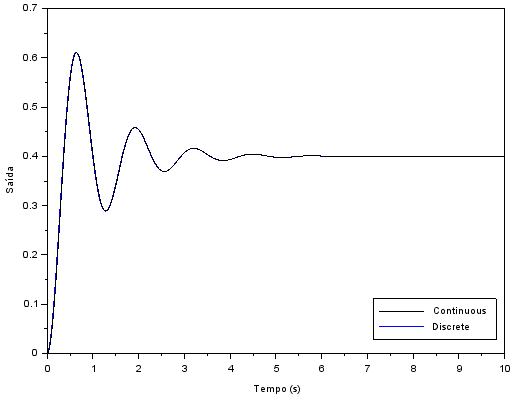
\includegraphics[width=7.5cm]{images/first_output/estavel_degrau.png}  
        \label{saida:est:deg}
    }
    \subfigure[Comparação]{                                              
        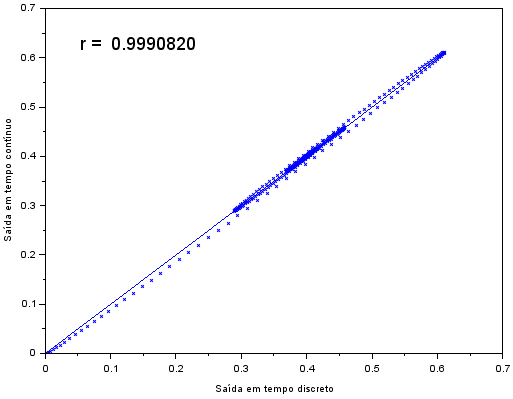
\includegraphics[width=7.5cm]{images/first_output/estavel_degrau_cor.png}
        \label{saida:est:deg:cor}
    }                
\end{center}
\caption{(a) Saída do sistema estável para uma entrada do tipo degrau e (b) comparação através de dados estatísticos das saídas no tempo discreto e contínuo}
\label{saida:est:1} 
\end{figure}


\begin{figure}[H]
\begin{center}
    \subfigure[Saída]{             
        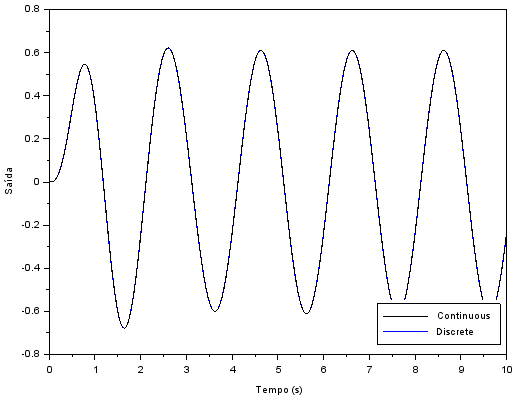
\includegraphics[width=7.5cm]{images/first_output/estavel_senoide.png}  
        \label{saida:est:sen}
    }
    \subfigure[Comparação]{                                              
        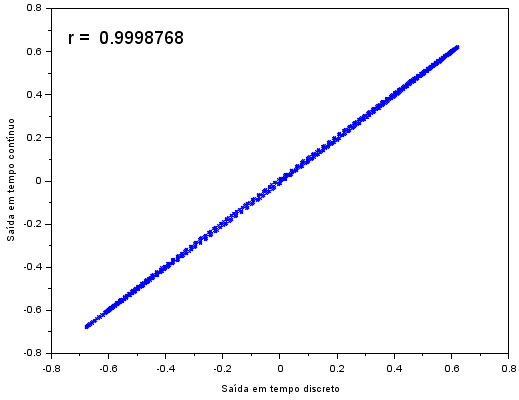
\includegraphics[width=7.5cm]{images/first_output/estavel_senoide_cor.png}
        \label{saida:est:sen:cor}
    }                
\end{center}
\caption{(a) Saída do sistema estável para uma entrada do tipo senoide (0.5Hz) e (b) comparação através de dados estatísticos das saídas no tempo discreto e contínuo}
\label{saida:est:2} 
\end{figure}


\begin{figure}[H]
\begin{center}
    \subfigure[Saída]{             
        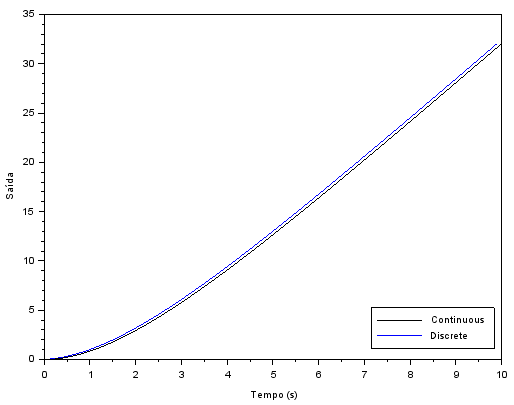
\includegraphics[width=7.5cm]{images/first_output/instavel_degrau.png}  
        \label{saida:ins:deg}
    }
    \subfigure[Comparação]{                                              
        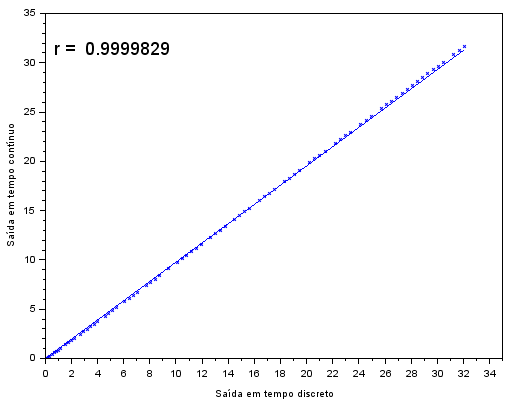
\includegraphics[width=7.5cm]{images/first_output/instavel_degrau_cor.png}
        \label{saida:ins:deg:cor}
    }                
\end{center}
\caption{(a) Saída do sistema instável para uma entrada do tipo degrau e (b) comparação através de dados estatísticos das saídas no tempo discreto e contínuo}
\label{saida:ins:1} 
\end{figure}


\begin{figure}[H]
\begin{center}
    \subfigure[Saída]{             
        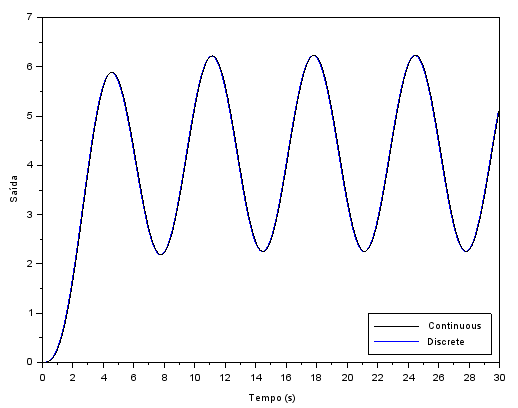
\includegraphics[width=7.5cm]{images/first_output/instavel_senoide.png}  
        \label{saida:est:sen}
    }
    \subfigure[Comparação]{                                              
        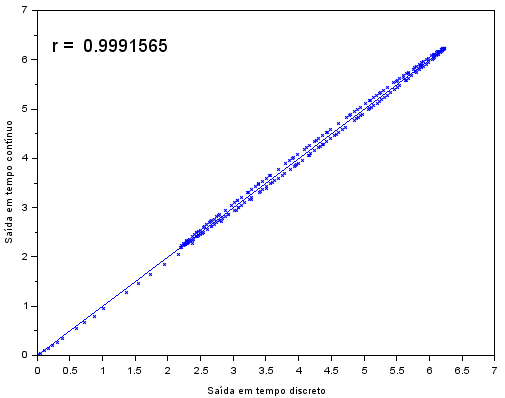
\includegraphics[width=7.5cm]{images/first_output/instavel_senoide_cor.png}
        \label{saida:ins:sen:cor}
    }                
\end{center}
\caption{(a) Saída do sistema instável para uma entrada do tipo senoide (0.15Hz) e (b) comparação através de dados estatísticos das saídas no tempo discreto e contínuo}
\label{saida:ins:2} 
\end{figure}

\pagebreak





